\documentclass{hw_template}

\title{\bfseries Контрольна Робота. Частина \#3}
\author{\bfseries Захаров Дмитро}
\date{30 листопада, 2024}

\begin{document}

\pagestyle{fancy}

\maketitle

\section{Завдання 1}

\begin{problem}
    Знайти розв’язок задачі синтезу
    \begin{equation*}
        \begin{cases}
            \dot{x}_1 = \mu x_1 + \nu x_2 + u_1, \\
            \dot{x}_2 = -\nu x_1 + \mu x_2 + u_2
        \end{cases}, \quad u_1^2 + u_2^2 \leq 1,
    \end{equation*}

    для $\mu=-3$, $\nu=6$. А саме:
    \begin{enumerate}
        \item Задати довільну початкову точку. Розв’язати в ній рівняння
        $2\mu\Theta-1+e^{-2\mu\Theta}=2\mu^2(x_1^2+x_2^2)$. Цей розв’язок і є
        часом руху. \textbf{(3б)}
        \item Підставити керування $\mathbf{u}(x_1,x_2)=\left(-\frac{\Theta(x_1,x_2)x_1}{x_1^2+x_2^2}, -\frac{\Theta(x_1,x_2)x_2}{x_1^2+x_2^2}\right)$ у початкову систему. Похідна 
        від функці керованості дорівнює $-1$. Розв'язати задачу Коші. \textbf{(3б)}
        \item Побудувати траєкторію керування 1 і 2. \textbf{(4б)}
    \end{enumerate}
\end{problem}

\textbf{Розв'язання.}

\textbf{Пункт 1.} Задамо, наприклад, $\mathbf{x}_0 = \left(\frac{1}{2}, \frac{1}{2}\right)$. В такому разі, маємо рівняння:
\begin{equation*}
    2\mu\Theta_T-1+e^{-2\mu\Theta_T}=2\mu^2(x_1^2+x_2^2) \iff -6\Theta_T+1+e^{6\Theta_T} = 9,
\end{equation*}

де $\Theta_T \in \mathbb{R}_{\geq 0}$ --- час руху. Це рівняння можна розв'язати
чисельно за допомогою \textit{Wolfram Mathematica}. Чисельно, отримуємо $\Theta_T \approx
0.42$. 

\textbf{Замітка.} Для відносно великих за модулем $\mu<0$ (як в нашому випадку),
можна вважати, що $e^{-2\mu\Theta_T} \gg 2|\mu|\Theta_T$ і тому наближено розв'язок 
можна знайти як $e^{-2\mu\hat{\Theta}_T} = 1+2\mu^2(x_1^2+x_2^2)$, звідки:
\begin{equation*}
    \hat{\Theta}_T = -\frac{1}{2\mu}\log(1+2\mu^2(x_1^2+x_2^2)).
\end{equation*}

Така оцінка дає $\hat{\Theta}_T \approx 0.38$ --- досить близьке значення до чисельного.

\textbf{Пункти 2-3.} Найбільша проблема цього пункту полягає у тому, що розв'язок
$\Theta(x_1,x_2)$ не є аналітично виразним. Тому, функцію $\Theta(x_1,x_2)$ ми знайдемо
чисельно. Проте, яким саме чином?

Ми знаємо, що увесь рух обмежений в квадраті $\|\mathbf{x}\|_1 \leq
\|\mathbf{x}_0\|_1$, тому достатньо згенерувати сітку на цьому квадраті
(скажімо, $\{(x_1^{(i)},x_2^{(i)},\Theta(x_1^{(i)}, x_2^{(i)}))\}_{i \in [N]}$) і
знайти значення $\Theta$ в кожній точці, розв'язавши відповідне рівняння. Приклад 
сітки зображено на рисунку \ref{fig:grid}.

\begin{figure}[H]
    \centering
    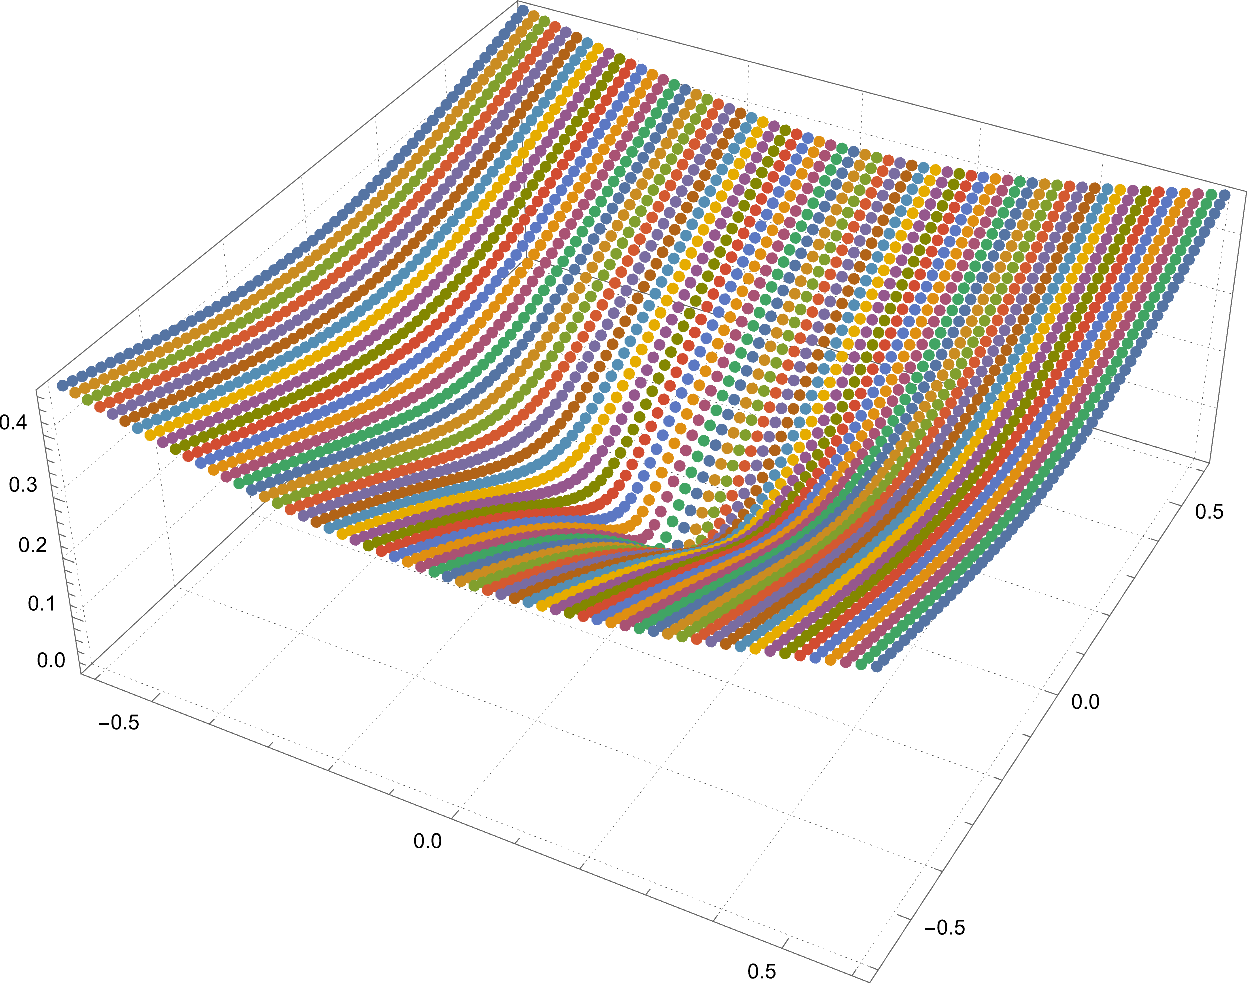
\includegraphics[width=0.6\textwidth]{figures/grid.pdf}
    \caption{Сітка $\{(x_1^{(i)},x_2^{(i)},\Theta(x_1^{(i)}, x_2^{(i)}))\}_{i \in [N]}$.}
    \label{fig:grid}
\end{figure}

Далі, цю сітку ми інтерполюємо або апроксимуємо якимось методом (наприклад, за
допомогою методу \texttt{Interpolate} в \textit{Wolfram Mathematica}). Таким
чином, ми отримуємо неперервно-диференційовану (навіть кілька разів) функцію
$\hat{\Theta}(x_1,x_2)$. Результат зображено на рисунку \ref{fig:theta}.

\begin{figure}[H]
    \centering
    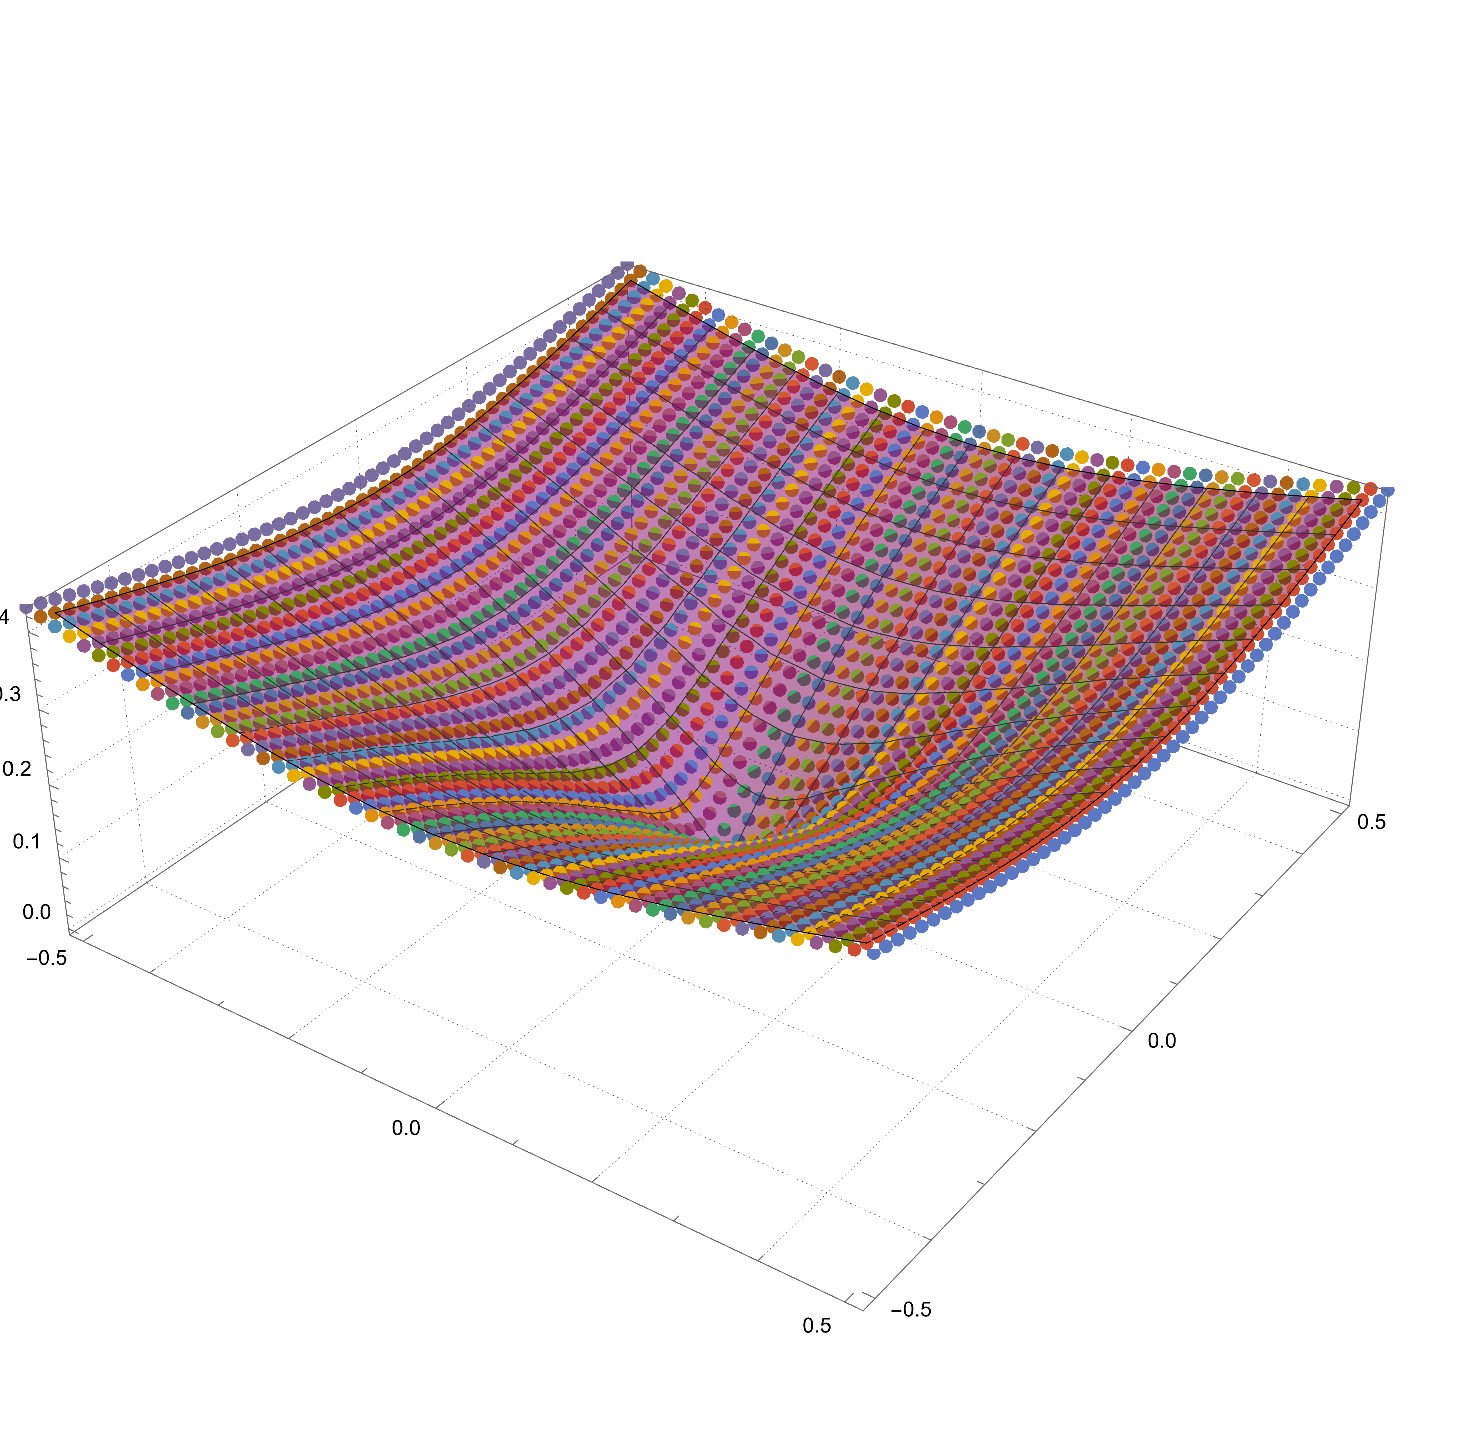
\includegraphics[width=0.6\textwidth]{figures/interpolation.pdf}
    \caption{Функція $\hat{\Theta}(x_1,x_2)$.}
    \label{fig:theta}
\end{figure}

Далі, як і каже умова, вибираємо керування:
\begin{equation*}
    \mathbf{u}(x_1,x_2) = \left(-\frac{\hat{\Theta}(x_1,x_2)x_1}{x_1^2+x_2^2}, -\frac{\hat{\Theta}(x_1,x_2)x_2}{x_1^2+x_2^2}\right).
\end{equation*}

І чисельно розв'язуємо задачу Коші для початкової системи. Траєкторія системи
зображена на рисунку \ref{fig:trajectory}. Зокрема, графіки $u_1(t)$ та
$u_2(t)$, а також $u_1^2(t)+u_2^2(t)$ можна знайти у доданому файлі
\textit{Wolfram Mathematica}.

\begin{figure}[H]
    \centering
    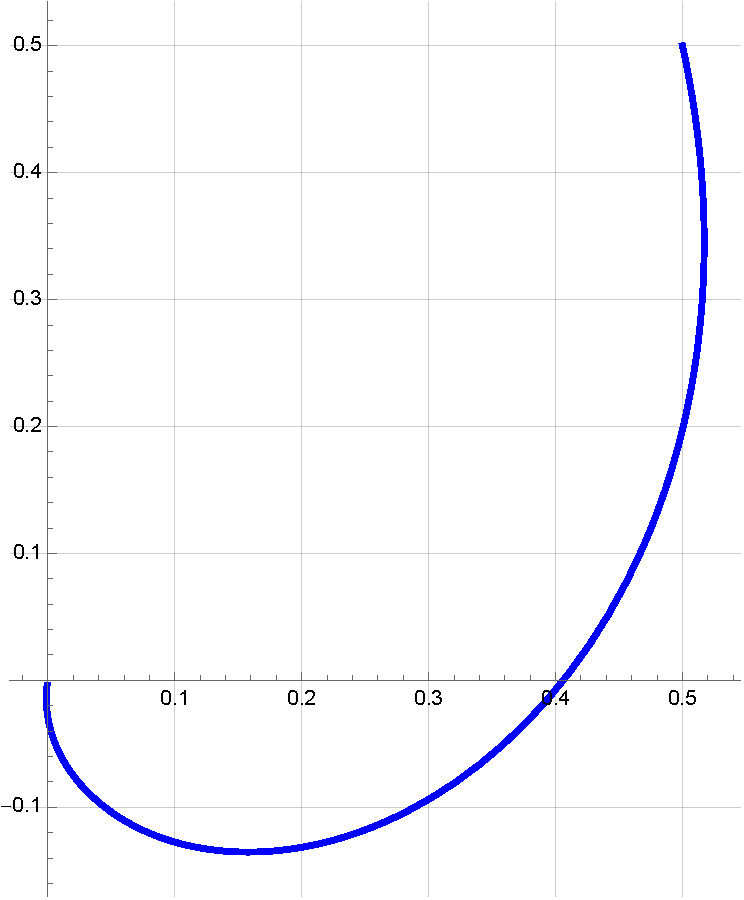
\includegraphics[width=0.6\textwidth]{figures/trajectory.pdf}
    \caption{Траєкторія системи.}
    \label{fig:trajectory}
\end{figure}

\newpage

\section{Завдання 2}

\begin{problem}
    Розглянемо наступну систему, де $\varepsilon=0.005$, $\delta=0.01$:
    \begin{equation*}
        \begin{cases}
            \dot{x}_1 = x_2 + \varepsilon(x_2^2+x_1u), \\
            \dot{x}_2 = u + \delta(x_1^2-x_2u)
        \end{cases}, \quad |u|\leq 1,
    \end{equation*}
    \begin{enumerate}
        \item Задати довільну початкову точку, яка належить заданій області
        $\mathcal{Q}=\left\{(x_1,x_2):3x_1^2+2x_1x_2+x_2^2\leq
        \frac{2}{9}\right\}$. Намалювати область (лінія рівня функції 
        $\theta$ при $\theta=1$). Потім взяти точку в середині і знайти 
        її координати. \textbf{(3б)}
        \item Розв'язати в цій точці рівняння $\frac{2}{9}\Theta^4 -
        \Theta^2x_2^2 - 2\Theta x_1x_2 - 3x_1^2 = 0$. \textbf{(3б)}
        \item Розв'язати задачу Коші 
        \begin{align*}
            \dot{x}_1 &= x_2 + 0.01\left(-\frac{x_1^2}{x_3^2}-\frac{2x_1x_2}{x_3}+x_2^2\right),\\
            \dot{x}_2 &= -\frac{x_1}{x_3^2}-\frac{2x_2}{x_3}+0.01\left(\frac{x_1x_2}{x_3^2}+\frac{2x_2^2}{x_3}+x_1^2\right),\\
            \dot{x}_3 &= \frac{x_1^2+x_3^2x_2^2}{6x_1^2+3x_3x_1x_2+x_3^2x_2^2} \\
            &+ \frac{(-3+x_3^3)x_1^3+x_3(-8+x_3^3)x_1^2x_2 - 2x_3^2x_1x_2^2-x_3^3x_2^3}{100x_3(6x_1^2+3x_3x_1x_2+x_3^2x_2^2)}, \\
            x_1(0) &= x_{10}, \quad x_2(0) = x_{20}, \quad x_3(0) = \Theta_0 
        \end{align*}
        Час руху знаходиться з умови, що $\sqrt{x_1^2+x_2^2}\leq 0.01$. \textbf{(3б)}
        \item Побудувати траєкторію, керування і похідну від функції керованості. \textbf{(4б)}
    \end{enumerate}
\end{problem}

\textbf{Розв'язання.}

\textbf{Пункт 1.} Власне, в цьому пункті малюємо область $\mathcal{Q}$ у
\textit{Wolfram Mathematica} і обираємо випадкову точку. Я, наприклад, обрав
$\mathbf{x}_0 = \left(0.2, -0.4\right)$. Легко переконатися, що $\mathbf{x}_0
\in \mathcal{Q}$. Результат зображено на рисунку \ref{fig:region}.

\begin{figure}[H]
    \centering
    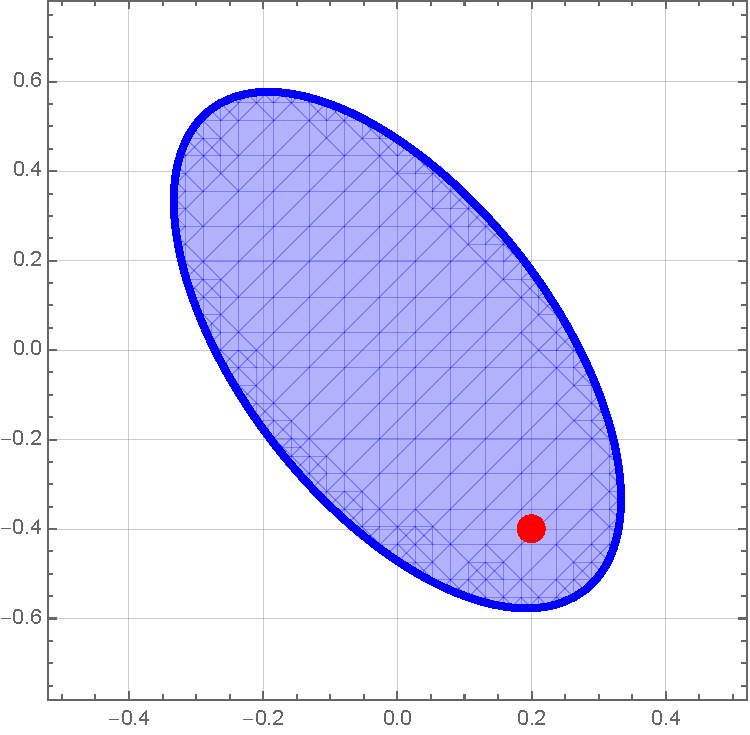
\includegraphics[width=0.6\textwidth]{figures/q.pdf}
    \caption{Область $\mathcal{Q}$.}
    \label{fig:region}
\end{figure}

\textbf{Пункт 2.} Чисельно розв'язуємо рівняння в цій точці:
\begin{equation*}
    \frac{2}{9}\Theta_0^4 - \Theta_0^2x_2^2 - 2\Theta_0 x_1x_2 - 3x_1^2 = 0 \iff \frac{2}{9}\Theta_0^4 - 0.16\Theta_0^2 + 0.16\Theta_0 - 0.12 = 0.
\end{equation*}

З цього рівняння можна знайти $\Theta_0 \approx 0.809$.

\textbf{Пункт 3.} З цього пункту починаються деякі труднощі. По-перше, без повного
аналізу параграфу, дуже складно зрозуміти, як перетворити рівняння, щоб воно 
включало нові параметри $\varepsilon$ та $\delta$. Тим не менш, моя інтуїція 
підказує на те, що рівняння стає наступним:
\begin{align*}
    \dot{x}_1 &= x_2 + \varepsilon\left(-\frac{x_1^2}{x_3^2}-\frac{2x_1x_2}{x_3}+x_2^2\right),\\
    \dot{x}_2 &= -\frac{x_1}{x_3^2}-\frac{2x_2}{x_3}+\delta\left(\frac{x_1x_2}{x_3^2}+\frac{2x_2^2}{x_3}+x_1^2\right),\\
    \dot{x}_3 &= \frac{x_1^2+x_3^2x_2^2}{6x_1^2+3x_3x_1x_2+x_3^2x_2^2} \\
    &+ \frac{(-3+x_3^3)x_1^3+x_3(-8+x_3^3)x_1^2x_2 - 2x_3^2x_1x_2^2-x_3^3x_2^3}{100x_3(6x_1^2+3x_3x_1x_2+x_3^2x_2^2)}, \\
    x_1(0) &= 0.2, \quad x_2(0) = -0.4, \quad x_3(0) \approx 0.809.
\end{align*}

Для нього я зробив програму, що розв'язує задачу Коші, будує траєкторію та функцію
керування. Отримав, що час руху приблизно $T\approx 1.74$ (в якості критерію
кінця руху, я взяв мінімальне $T$, за яке $\sqrt{x_1(T)^2+x_2(T)^2}\leq 0.01$,
згідно умові). Результат зображено на рисунках \ref{fig:trajectory2} та
\ref{fig:control}.

\begin{figure}[H]
    \centering
    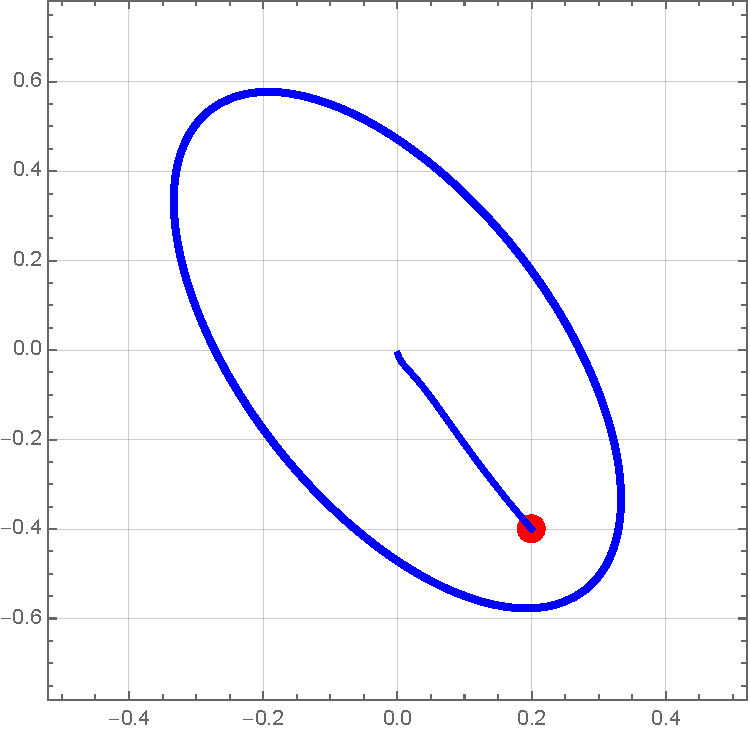
\includegraphics[width=0.6\textwidth]{figures/trajectory_2.pdf}
    \caption{Траєкторія системи.}
    \label{fig:trajectory2}
\end{figure}

\begin{figure}[H]
    \centering
    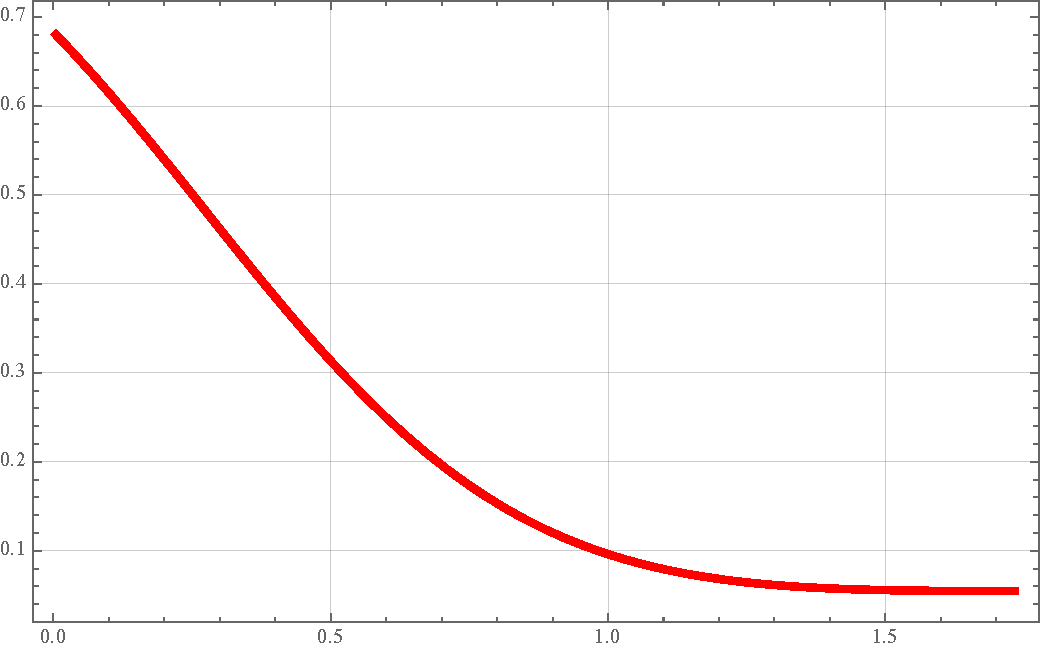
\includegraphics[width=0.6\textwidth]{figures/control.pdf}
    \caption{Функція керування $u(t)$.}
    \label{fig:control}
\end{figure}

Проте, оскільки я не впевнений у правильності рівняння, я вирішив розв'язати задачу
заново, користуючись наступним алгоритмом:
\begin{enumerate}
    \item Розв'язати рівняння $\frac{2}{9}\Theta^4 - x_2^2\Theta^2-2\Theta x_1x_2-3x_1^2=0$ на певному наборі точок
    на квадраті $[-0.8,0.8] \times [-0.8,0.8]$.
    \item По отриманним точкам побудувати інтерполяцію $\hat{\Theta}(x_1,x_2)$.
    \item Побудувати функцію керування як $u(x_1,x_2)=-\frac{x_1}{\hat{\Theta}^2(x_1,x_2)}-\frac{2x_2}{\hat{\Theta}(x_1,x_2)}$.
    \item Підставити керування у початкову систему та розв'язати задачу Коші.
    \item Побудувати траєкторію системи, керування та похідну від функції керованості.
\end{enumerate}

Результати додані у програмі \textit{Wolfram Mathematica}. З цікавого, функція 
$\dot{\Theta}$ виглядає доволі екзотично --- дивись рисунок \ref{fig:theta_dot}.

\begin{figure}[H]
    \centering
    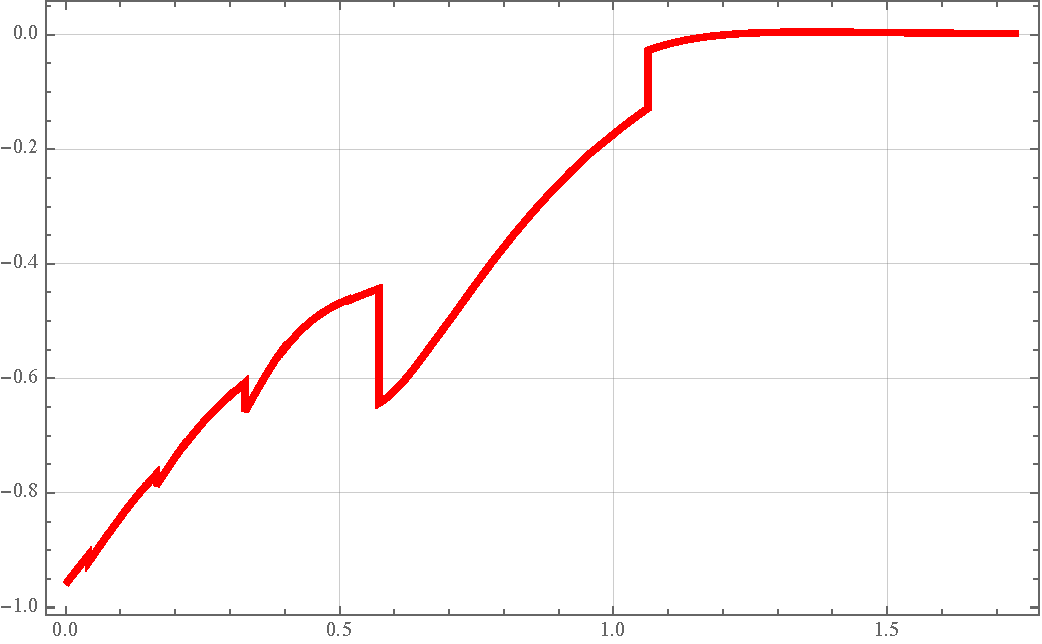
\includegraphics[width=0.6\textwidth]{figures/theta_dot.pdf}
    \caption{Похідна від функції керованості $\dot{\Theta}(\mathbf{x}(t))$.}
    \label{fig:theta_dot}
\end{figure}

\end{document}